\documentclass[]{article}
\usepackage[margin=2.8cm]{geometry}
\usepackage{amssymb}
\usepackage{filecontents,hyperref}
\usepackage[style=authoryear, backend = bibtex,maxcitenames=2]{biblatex}
\usepackage{graphicx}
\usepackage{afterpage}
\usepackage{caption}
\usepackage{float}
\usepackage{chngcntr}
\usepackage{algorithm}
\usepackage[noend]{algpseudocode}
\usepackage{listing}

\newcommand\blankpage{%
    \null
    \thispagestyle{empty}%
    \addtocounter{page}{-1}%
    \newpage}

\let\oldsection\section
\renewcommand\section{\clearpage\oldsection}

\newenvironment{changemargin}[2]{%
\begin{list}{}{%
\setlength{\topsep}{0pt}%
\setlength{\leftmargin}{#1}%
\setlength{\rightmargin}{#2}%
\setlength{\listparindent}{\parindent}%
\setlength{\itemindent}{\parindent}%
\setlength{\parsep}{\parskip}%
}%
\item[]}{\end{list}}

\def\code#1{\texttt{#1}}

%opening
\large
\title{Game Playing AI for Settlers of Catan
\\ \textit{Project Report}}
\author{Student: David Martin 
\\ Supervisors: Dr Lars Kunze & Dr Nick Hawes}
\date{}
\bibliography{report.bib}
\addbibresource{report.bib}

\begin{document}


\begin{titlepage}
    \begin{center}
        \vspace*{1cm}
        
        \textbf{Game Playing AI for Settlers of Catan}
        
        \vspace{0.5cm}
        
        \vspace{1.5cm}
        
        \textbf{David Martin} 
        \\
        \textbf{Supervisors: Dr Lars Kunze and Dr Nick Hawes}
       	
       	\vspace{1.5cm}
       	
        
\includegraphics[width=0.5\textwidth]{images/logo}
  
		\vspace{1.5cm}  
  
        \parbox[][][c]{0.5\textwidth}{\centering Submitted in conformity with the requirements
                       for the degree of BSc Computer Science
                       School of Computer Science
                       University of Birmingham}

     
       
        
        \vfill
        
        \vspace{0.8cm}
        
        
       	School of Computer Science\\
        University of Birmingham\\
       
        
    \end{center}
\end{titlepage}

\blankpage

\thispagestyle{plain}
\begin{center}
    \huge
    \textbf{Abstract}
    \\
    \large
    \vspace{1.0cm}
    \textbf{Game Playing AI for Settlers of Catan}   
    \vspace{0.2cm}
    \\
    David Martin
    \vspace{0.1cm}
    \\ 
    \noindent\makebox[\linewidth]{\rule{\textwidth}{1pt}} 
\end{center}

\pagenumbering{roman}

\begin{changemargin}{1.8cm}{1.8cm}
 Game Playing is both a useful and important way of measuring the performance of artificial intelligence techniques. Commonly these developments are tested on games such as Chess, Backgammon, or more recently, Go. While these games are very well researched and explored there are many other games that have not yet been utilised to the same level but provide very interesting characteristics and 
 features that make them worthy of further study.
 
 In this project, we designed and implemented a ``bot" that is capable of playing the popular board game Catan, also popularly known as Settlers of Catan. This game is interesting as a number of different characteristics make it somewhat unusual and harder in terms of the methods that must applied to play it than games regularly used for the development of AI.1
 
 By building on past work on AI for this game, a system is developed that relies on Monte Carlo Tree Search at its core and also utilising applied heuristics in order to play the game to a strong level, given enough time to calculate its ideal move.
 
 A set of tests are then run against a baseline AI showing that the bot developed in this work performs well when tested over a number of games and is capable of effective play against an average human player and respectable play against an expert one, although it remains evident that there are obvious improvements that could be made to our system which would further boost its performance, the results are thus far are highly promising
\end{changemargin}


\pagebreak

\thispagestyle{plain}
\begin{center}
    \huge
    \textbf{Acknowledgments}
    \\
    \large
    \vspace{0.5cm}
    \noindent\makebox[\linewidth]{\rule{\textwidth}{1pt}} 
\end{center}

\begin{changemargin}{1.8cm}{1.8cm}

I would like to thank my supervisors Dr Lars Kunze and Dr Nick Hawes for their advice and guidance without which this project would not have been possible.

\vspace{0.2cm}

Additionally, I would also like to thank Jeremy Monin, the maintainer and lead developer of the open source JSettlers2 program, which provides the engine for my project, for helping me with guidance on the usage of the program and for incorporating helpful changes into the software. Without this software the project would not have advanced as far in the time available.


\end{changemargin}
\pagebreak

\begin{center}
\Large \centering Declaration
\end{center}

\par The material contained within this thesis has not previously been submitted for a degree
at the University of Birmingham or any other university. The research reported within this
thesis has been conducted by the author unless indicated otherwise.

\tableofcontents

\pagebreak

\pagenumbering{arabic}

\section{Introduction}
\subsection{Game Playing}
 While at first the idea of game playing may seem irrelevant to the development of AI, upon further inspection it transpires that work on this area not only helps to progress the field of artificial intelligence but it also provides a way in which various techniques can be effectively tested and evaluated in a controlled environment.

\par Board games are most commonly used for this area of research as they can be easily represented using a computer, with their rules changed or the environment modified. Several different games are commonly used for research into game playing AI thanks to the different features that each games possesses. Perhaps the most ubiquitous game in this field is Chess, which has seen significant research effort spent since at least the late 1950s. Chess provides a good choice for the development of basic game AI as it is a game of perfect information, contains only one opposition player and has a very rich source of expertise surrounding the game while at the same time being complex, with a large enough branching factor that the game could not be solved using brute force methods alone.

\par Backgammon is also commonly used in the field of game playing AI. It shares most of the features if Chess, but at the same time introduces an element of chance through the usage of dice. This adds further complications to the techniques used to play the game.

\par Despite the relative complexities of these games, AI has been developed to play both backgammon and chess beyond the level of the best human players \cite{tesauro1995temporal, campbell2002deep}. The best chess bots have been unable to be beaten by humans for a number of years now and backgammon theory was significantly advanced by the development of AI which played the game using methods and strategies previously unseen by human players.

\par More recently focus in this area has shifted to applying new techniques to games that had previously not seen top level humans beaten by robots on a consistent basis, such as Go and Poker. Go being particular popular at the moment due to its incredibly large branching factor when compared to chess as well as other factors \cite{burmeister1995challenge}

\par On top of its relevance to the development of game playing, artificial intelligence also has strong applications in other fields such as game theory, which provides the mathematical basis behind much of the research in this area, and economics. In an economic scenario economies can be modelled as games with the different agents in the system competing and cooperating in order to maximise their own gain.

\par In this project we design and implement an AI that can play the popular board game Catan, designed by Klaus Terber and originally published by Mayfair Games. This game features elements that are considerably more complex that both chess and backgammon. The number of moves that can be played on any given turn is generally larger, and like backgammon there are dice rolls which introduce non-determinism into the game. Further complications are added by the multi-player nature of the game as 4 people play it at once, imperfect information, randomisation of the board and player-to-player trading. All aspects of a game that are not in Chess or Backgammon. While bots exists for Chess, Backgammon and recently, Go and Poker, that can beat the best human players, to our knowledge, there does not exist a bot that can yet consistently defeat the best Catan players in the world.
 
\subsection{Related Work}
In comparison to other more recently fashionable games, Catan has received only a small amount of attention from researchers. This is mostly due to the fact that rule set of the game is considerably more complex than that of the aforementioned games making it harder to implement in a computer setting. In these other games, while the strategy of playing the game may be equally as hard the rules are generally very simple to implement on a computer, with chess for example being able to be represented in a mere 455 bytes of data, and Go being able to be represented in an amount that is not considerably higher.

\par Despite the relative complexity of the rules of Catan, there do exist open source implementations of the game which can be used to run the game engine and enable the design of bots that can play the game. \textcite{szita2009monte} describes how a game of Catan can be played by utilising Monte Carlo Tree Search (MCTS). This paper shows that it is possible for MCTS to produce good results against bots using more naive, heuristic only approaches. The work does not however  extend much into the strategy employed by the MCTS, neglecting to mention how moves were generated for the MCTS. Details of the implementation of the MCTS are somewhat vague with little information given about how the problem of non-determinism is tackled within the tree search. There are also certain adjustments made to the rules of the game. For example, certain aspects of the game such as the imperfect information are removed, with all aspects of the game presented in a face up manner creating a game of perfect information.

\par \textcite{roelofs2012monte} also uses a Monte Carlo tree search to play the game. This paper can be seen to build upon the earlier work by Szita, and further explores the possibility of playing the game using MCTS. Of note in this particular work is the exploration of the different possibilities that present themselves for the node selection strategy and also for the final move choice. The work also presents useful methods for breaking down the tree search into groupings in order to improve speed and to help combat the issues that this study had with not being able to run enough simulations due to simulation performance. Results of the output from this paper were comparable to previous attempts to play this game using MCTS.

\par Further work relating to the development of a bot capable of playing Catan is provided by \textcite{pfeiffer2004reinforcement} who develops a bot using reinforcement learning techniques. The method employed involves creating a set of high level strategies which can be selected depending on the state of the game. These strategies are then used as heuristics to help guide the learning process for a self playing game which shows increased performance as a result of the learning process. The competency of the AI in this particular area is hard to judge as it is only really tested against a human player of which the skill level is unknown, though it would appear that this bot performs somewhat less effectively than the bots presented by \textcite{szita2009monte} or \textcite{roelofs2012monte} yet still achieves an acceptable level of play.

\par Additional work exploring AI for Catan is by \textcite{thomas2003real}. The approach in this work is considerably different from the attempts which attempt using MCTS to play the game. Notably this work is based on a series of heuristics and high level strategies, drawing parallels to Pfeiffer's work. However, there is no reinforcement learning, with a focus instead on low level heuristics to achieve the goals set out by a high level plan. The AI developed as a result of this paper is the basis of the AI in a large number of web servers that host the game as part of the JSettlers platform. Its efficiency is noteworthy, with decisions of what move to play happening almost instantly, in a very short space of time.

\par A paper by \textcite{branca2007using},explores a multi agent heuristic driven approach to playing Catan. Notably, this work shows that their developments are not able to beat monolithic solutions with a single decision making unit, perhaps suggesting that this approach may be less effective than others examined. In particular, the AI struggled with the long planning that is required to control the game but did make good short-term decisions. Of interest in this paper however is the ability of the bot to trade with other players, a feature that is commonly missing from other attempts to play Catan.

\par Other published studies are less focussed on the development of a bot that can play the game in a stand alone manner but are interested in aspects like determining optimal strategies for trading between players and analysing the most likely moves that a player could expect. For example a paper by \textcite{afantenos2012developing} analyses the conversations that occur between players and how this influences trading in the game.

\par More papers describing attempts to develop AI bots are difficult to find. Upon an analysis of the literature surrounding this game it appears that there are three main approaches taken to developing bots to play this game; heuristic systems, MCTS based systems and other reinforcement learning systems. It should be noted however, that most techniques, though mainly belonging to one of the above, also commonly integrate features of the others and in fact it could be argued that MCTS is simply a form of reinforcement learning with the search training itself on policy through the Monte Carlo simulations.

\subsection{Aims}
The aim of this project was to build upon previous research into AI for Catan and to design a bot that performs at a strong level. This could be classified by winning a high proportion of its games against bot opponents and scoring a high number of victory points in those games that it is not capable of winning. It was also desirable to be able to play against an expert human opponent in a ``convincing'' manner with the strong possibility of winning these games.

\par Previous efforts to design AI for Catan has found that even when other AI software has been able to be defeated by any developments made, expert human players have been comfortably able to beat any proposed solutions. 


\subsection{Report Structure}

\vspace{0.3cm}

\paragraph{\large Introduction}-
\vspace{0.2cm}
\newline In this section we introduce the project as a whole and give information regarding the work related to this project as well as the aims and motivation behind it.

\paragraph{\large Background}-
\vspace{0.2cm}
\newline In this section of the report we discuss the background information regarding the project. This includes information about the game of Catan and its rules and strategies as well information about the possible AI techniques that could be used to develop this software.

\paragraph{\large Implementation and Development}-
\vspace{0.2cm}
\newline This section details the decisions taken during the development of the project and the implementation that was followed in order to enact those designs.

\paragraph{\large Results}-
\vspace{0.2cm}
\newline In this section the results of a number of different tests on the system to measure to effectiveness and impact of numerous aspects are carried out. Details of the test environment are also given. 

\paragraph{\large Evaluation}-
\vspace{0.2cm}
\newline This sections draws upon the results gathered in order to evaluate the effectiveness of the system and to what degree it met the aims specified

\paragraph{\large Conclusion}-
\vspace{0.2cm}
\newline In this section conclusions are drawn on the project, including any future work that could be completed.

\section{Background}
In order to better understand the game and the rationale behind the project, details of the game and its various components are hereby discussed in the subsequent sections. 


\subsection{Catan}
Catan is a popular boardgame designed by Klaus Terber and first published in 1995. The game is considered a ``Eurogame'' a class of game often also described as ``German Style''. The focus in this style of game is to put emphasis on player communication and skilful play. This could, perhaps, be contrasted with other board games with more emphasis on conflict between payers such as Risk or games where luck plays a much larger role in the proceedings such as Monopoly. 

\par While comparing it with other games it is important to note that Eurogames such as Catan normally involve less skill based play than the more abstract and traditional games of Go and Chess; this is mainly owing to the absence of chance in these games, as well as the general lack of communication and interaction between players when it comes to the decision making process.

\par In addition to the basic game that has been released, there have been a number of optional expansions added to the base game which provide the opportunity for more players to join the game at once, as well as allowing more complex and interesting scenarios to explored. For the purposes of this project we only used the basic game played with 4 players and the most up to date version of the official rules.

\par Since its release the game has sold more than 22 million copies and been translated into at least 30 different languages \autocite{variety2015}. Catan has also won numerous awards including the German ``Speil des Jahres'' (Game of the Year) award and in 2005 was added to the Hall of Fame of the Games 100 buyers guide at the earliest opportunity (\citeauthor{spielDesJahr}) indicating its status as a critically acclaimed and popular title.

\subsection{Rules of the Game}
The rules of Catan are reasonably complex yet at the same time easy to understand. The following section will attempt to explain the rules of the game. If the reader already understands the rules then it is recommended that this section is skipped. An official source of the rules can be obtained from the Catan website. (http://www.catan.com/service/game-rules)

\subsubsection{The Board and Playing Equipment}
The board of Catan consists of 37 hexagons, tessellated to form a single larger hexagon where each edge consists 4 of the smaller pieces. The outer ring of hexagons on the board make up the tiles representing the sea. These tiles are considered out of bounds and nothing can be built on them.

\par Each tile on the board that is not in the sea has a number and resource associated with it. These are the terrain hexes and there are 19 of them. The number on the tile corresponds to a possible result of a double dice roll. No tile on the board has the number 7 on it. One tile in the board has no resource or number on it and is referred to as the desert. For each game the position of these tiles and the numbers on them is randomised, although some sort of agreement may be reached regarding the quality of a layout between players.

\par The board can therefore be thought to be made up of a number of hexes, nodes and edges. Hexes are the large hexagon shaped pieces which normally have a number and resource placed on them. Around each hexagon are 6 nodes, one on each vertex. These nodes are the positions at which settlements and cities in the game can be placed. Each of these nodes is adjacent to at most 3 and at least 1 labelled hex. Edges are the connections between two nodes and can have roads built on them during the game.

\par There are 5 different types of resource in the game. Each is required by the player to perform various actions in the game such as building. Alternative names for the resources are sometimes used and are provided for reference. In this report the first term listed will be used throughout.
\begin{itemize}
  \item Clay (Brick) - 3 Hexes
  \item Wood (Lumber)- 4 Hexes
  \item Wheat (Grain) - 4 Hexes
  \item Sheep (Wool) - 4 Hexes 
  \item Ore (Stone) - 3 Hexes
\end{itemize}

\par Around the board there are a number of ports. These ports are located in the sea hexes and there is one port for each resource as well as 4 generic ports to give a total of 9. These ports are attached to either one or two territories and are used for certain types of trades by the player.

\par Each of the 4 players in the game has an equal number of pieces that can be placed on the board. There is a fixed limit on the number of pieces of each type that a player can place onto the board determined by the number of physical pieces that they possess. 

\begin{itemize}
  \item Road - 15 Pieces
  \item Settlement - 5 Pieces
  \item City - 4 Pieces
\end{itemize}


\par Not owned by the players are a deck of 25 development cards. These cards are shuffled before the game to randomise the order of them. Also not possessed by the player is a bank of resource cards, which should be handed out as and when necessary by a nominated player.

\subsubsection{Beginning the Game}
At the start of the game one of the players is chosen randomly to go first and play then proceeds in a clockwise direction. The start phase of the game of Catan is then initiated. This phase has notable differences to the rest of the game. In turn, each player places one settlement and one road on the board for free. The settlement may be placed on any legal node of the board. The road must be placed on one of the edges connecting to the node the settlement was placed on. After the 4th player has placed their road and settlement on the board then the second phase of the opening begins. The 4th player that has just placed their pieces then moves again and places another settlement and road. The settlement can again be placed in any legal location and the road must also be attached to the node the settlement was placed on. During this second phase however the player will also receive one of the corresponding type for each hex the settlement was adjacent to. This means that a maximum of 3 resources and a minimum of one resource can be obtained. This continues until the play has returned to the first player. A total of 8 settlements and 8 roads will have been placed over the board and regular play now commences from the first player and continues until the end of the game.

\subsubsection{Regular Turn}
During a regular turn a player begins by rolling the dice. The result of the dice roll will correspond to a value on the board with the exception of a 7. Resources are then distributed with each settlement adjacent to a hex with the rolled value on earning the owner 1 of the type of resource pictured on the tile. Cities earn the player two resources. It is possible for a player to own multiple structures around a single hex in which case they receive the number of resources corresponding to the structures around it.

\par After the dice has been rolled the player may spend any amount of time spending their resources to build or buy. They may also perform an unlimited amount of trades with other players or the bank. When a player is satisfied they may end their turn, resulting in play transferring to the next player in a clockwise direction. This type of turn continues until the game is won.

\subsubsection{Building}
On their turn a player may wish to spend their resources on building which allows them to place a piece onto the board. Any number of pieces may be placed in a single turn as long as the player has the piece to place and the correct number of resources. There are rules regarded the positions that each piece may be placed in:

\begin{itemize}
  \item Road - 1 Clay, 1 Wood - Must be placed on an edge that does not already contain a road and is connected on at least one end to another of the players roads, settlements or cities. It may not go through an opponents city or settlement.
  \item Settlement - 1 Clay, 1 Wood, 1 Wheat, 1 Sheep - Must be placed on a road owned by the player. There must be a gap of at least 2 edges between the settlement being placed and any other settlement or city.
  \item City - 3 Ore, 2 Wheat - Must be placed on a settlement. The settlement piece is returned to the player after the city piece is placed.
\end{itemize}

\par Building may only take place during the turn of the player placing the pieces.

\subsubsection{The Robber}
The board has a robber piece on it that starts in the desert hex. After a 7 is rolled the robber must be moved to another hex by the player that has rolled the 7. If there are settlements or cities around the hex that the player has chosen to move the robber to then the they may choose to steal a single resource from any of the owners of those structures. This resource is chosen randomly from the players hand. If there are no structures in the hex or the players that could be robbed do not currently own any resource cards then no resource shall be taken.

\par While a hex the robber located on it then it shall not produce any resources. Any time the number is rolled which corresponds to the value of the hex the robber is situated in then resources will not be given out to the owners of the surrounding settlements and cities.

\par If any player owns more than 7 cards when a 7 is rolled by any player they must give up half of their resource cards (rounded down) to the bank before any play continues. This rule is in place to stop players from hoarding resources. 

\subsubsection{Development Cards}
As well as building a player may also spend their resources on development cards:
\begin{itemize}
	\item Development Card - 1 Wheat, 1 Sheep, 1 Ore - If there are still cards remaining in the deck.
\end{itemize}

\par There are 5 different types of development card:

\begin{itemize}
	\item Knight (Soldier) - 14 Cards - Move the robber and rob a resource
	\item Victory Point Card - 5 Cards - Add one victory point to your score
	\item Monopoly - 2 Cards - Nominate a resource - receive every card of the resource held by the rest of the players
	\item Road Building - 2 Cards - Place two road pieces for free
	\item Year of Plenty - 2 Cards - Receive any two resource cards from the bank.
\end{itemize}

\par A development card may be played at any time during a players turn, even before the dice has been rolled. Only one development card may be played on any given turn. This means, for example, that if a player plays a knight card before the dice is rolled that they may not play any other development cards they possess after they have rolled the dice. A player may buy any number of development card on their turn.

\par The victory point development card is an exception to the above restrictions on playing development cards. They may be played at any time, remain hidden until playing them would end the game and are not limited to having only one able to be played at a time.

\subsubsection{Trading}
When it is their turn a player may decide to initiate a trade. Trades may be made either with the other players or with the bank.

\par When trades take place with other players any combination of resources may be offered in return for any others being received. Development cards may not be traded. A player may only directly initiate a trade during their turn though it often transpires that in games between 4 human players in a live setting that this rule is often relaxed.

\par A player may also trade to the bank. When trading to the bank a specific number of the same type of resource are traded for a single one of the trading player's choice. The number of resources that must be traded to the bank to receive a resource is initially 4. This number can however be reduced by utilising the ports around the edge of the board. If a settlement or city is located next to one of these ports then they are said to belong to the player. If a player owns a generic port then the number of resources reduces to 3 for all types of resource. If a port displaying a specific resource is owned then the number required for that type of resource only is reduced to 2.

\par There is no obligation to accept a trade or ensure that trades are fair. However, all trades to the bank will be accepted as long as the correct amount of resources are given.


\subsubsection{Winning the Game}
A game of Catan is won when a player reaches 10 Victory Points. These points are obtained in a number of different ways. There are 3 ways that provide permanent victory points

\begin{itemize}
	\item Settlements - Each settlement grants the owner 1 victory point
	\item Cities - Each city grants the owner 2 victory points
	\item Victory Point Cards - Each one owned by the player grants them 1 victory point. They remain hidden until they can be used to win the game or the game is over.
\end{itemize}

\par As well as these methods to gain permanent victory points there are also transient victory points which transfer between players as the game progresses.

\begin{itemize}
	\item Longest Road - The player with the longest road of at least 5 pieces gains 2 victory points. Branches and loops are not counted in this total
	\item Largest Army - The player with the most knight cards played and has placed at least 3 gains 2 victory points
\end{itemize}
 
 \par These victory points can be transferred to another player by them building a longer road or playing more knight cards than the player that currently has them.


\subsection{Catan Strategy}
In order to understand the development of a bot that can play Catan using AI techniques it is worth trying to understand the strategies and principles that human players normally use when playing the game. 

\par While there has been some work on trying to analyse Catan by applying Game Theory practices to it with notable work  by \textcite{guhe2014game} in attempting to empirically analyse certain strategies and also by \textcite{keep2010} who attempts to use mathematical theories to analyse gameplay and derive facts about the game. It is, however, clear that there is little work done on formally attempting to solve or analyse the game. This could be contrasted to games like checkers and connect four which have been solved.

\subsubsection{General Principles}
There are certain key principles that are generally followed during the game of Catan. Most obvious and important is the need to maximise the income of resources that a player receives throughout a game. Principally this is achieved in two different ways. Firstly this is done by making sure that settlements built are placed on nodes adjacent to hexes that are rolled more frequently. For example a 2 or 12 can only be produced in one way by two dice while an 8 or 6 can be rolled 5 different ways. A table is provided below of the probabilities of these rolls taking place. Secondly, resource gain is increased by building more settlements and cities. It is generally taken that they should be built whenever possible in order to increase the flow of resources for a player. A minor consideration that should also be taken into account is the spread of different values covered; if a player can place their settlements so that they cover a wide variety of values then they will make their flow of resources more consistent, allowing for fewer missed opportunities during turns.

\vspace{0.2cm}

\begin{center}


\begin{tabular}{|c|c|}
\hline 
2 & 2.778\% \\
\hline 
3 & 5.556\%\\
\hline 
4 & 8.333\% \\
\hline 
5 & 11.111\% \\
\hline 
6 & 13.889\% \\
\hline 
7 & 16.667\% \\
\hline 
8 & 13.889\% \\
\hline 
9 & 11.111\% \\
\hline 
10 & 8.333\% \\
\hline 
11 & 5.556\% \\
\hline 
12 &2.778\% \\
\hline 
\end{tabular}
\captionof{table}{Probabilities for 2 6-Sided Dice}
\end{center}

\vspace{0.2cm}

\par Another   crucial aspect regarding resources is to ensure that a player has a good spread of different types of resources. If a player is too focussed on few resource types then they will not be able to progress at the same rate that another player is as they will need to trade in order to make up for the shortage in resources.

\par Also important is that the resources a player possesses are constantly being spent. This is important for two main reasons. If a player hoards resources then they run the risk of having to discard half of them if the robber is activated, wasting them. Additionally, if a player holds resources rather than spending them they are wasting the opportunity to gain from those resources. 

\par A further key principle that should be observed is the synergy of certain types of resources with one another. Everything that can be purchased with wood also involves clay to be built and everything that can be purchased with ore also requires wheat. This means that it can be very effective to make sure that we try and keep these resources in pairs as they tend to be considerably less effective without their complimentary resource.

\par The relative value of different resources also changes throughout the course of the game. Clay and wood are generally considered to be early game resources, as they are vital for the building of roads and settlements which are generally placed at the beginning of a game. Wheat and Ore and are necessary for building cities and buying development cards which tend to be more useful as a game approaches its conclusion. All of these factors must be taken into account when deciding on the location and choice of resource deployment.

\subsubsection{Common Human Strategies}
When playing the game there are certain strategies that are commonly followed and recommend to new human players of the game. These strategies are generally the ones that are implemented when bots are designed that attempt to capture the tactics and strategies adopted by expert human players.

\par There are, generally speaking, 2 main strategies that are employed by most players in the game. The first of these is the wood and clay strategy, which normally ensues if a player has a strong income source of wood and clay. When following this strategy focus is placed on rapidly expanding the number of settlements that the player owns as well their roads. A main objective of this particular strategy is to obtain the victory points for owning the longest road. The large amount of roads that can be placed also allow the opportunity to control large sections of the board and block opponents off. This strategy generally becomes weaker later in the game where the maximum number of roads and settlements have been placed, rendering the initial investment in wood and clay eventually ineffectual. It is important that the expansion settlements built fill the voids in resource production left from focussing on clay and wood.

\par In contrast to the wood and clay strategy, is the ore driven strategy. This particular method involves focussing primarily on ore and also on wheat. The motivation behind this technique is to upgrade settlements to cities and also to purchase development cards. While the brick and clay strategy focusses on getting the longest road this methods eschews that and instead focusses on getting victory points from development cards, both through the victory point cards directly and also from the largest army victory points which results from playing the knight cards the player obtains. This strategy tends to be more effective during the late stage of the game, where the opportunities to build new roads and settlements would be limited but there are plenty of development cards remaining.

\par Naturally a hybrid strategy also exists, focussing on a mixture between the two aforementioned strategies. Generally, this involves getting a good mix of all of the resources and trying to balance building roads and settlements, with upgrading those settlements to cities and buying development cards. This strategy is more opportunistic that the other two with less emphasis placed on obtaining the largest army or longest road victory points that correspond to the other two strategies. 

\par It is important to note that these strategies must be flexibly chosen, and that it is not possible to decide on a particular course of action before the layout of the board is seen and the order of play determined. Only after this information and the knowledge of other players actions is taken into account is it possible to determine a strategy that will be played, this presents difficulties from an AI perspective as it will not be possible to hard code a single effective strategy into a bot which it can follow.

\subsubsection{Opening Turn}
Particularly crucial in Catan is the opening moves played each player at the start of the game. These opening moves result in two settlements and two roads being placed, for free, for each player and decide the strategy that will adopted by the them for a considerable portion fo the game. 

\par As these settlements can be placed in any legal location on the board without the requirement for roads it is important to ensure that a good position for the settlements is chosen. Ideally this should be occupying as many commonly rolled values as possible and should also be on resources that work well together.

\par Unlike other aspects of the game the strategy that should be employed in this section of the game is possible to capture with a set of rules and can be described in a mechanical fashion. This could be helpful, considering the differences in this stage of the game compared to other parts.

\subsubsection{Robber Strategy}
A further subsection of the strategy of the game that must be considered is the placement and usage of the robber piece. 

\par One part of this aspect of the game is deciding on where to position the robber when the player rolls a 7 or plays a knight card. Clearly, a player will not wish to deprive themselves of resources, except in very rare and specific situations. Normally the piece is placed so that the maximum amount of disruption to a players resource collection is caused. This is worked out by taking into consideration the likelihood of the value on that particular hex being rolled, as well as the number of structures around the nodes of that hex.

\par When moving the robber to a different hex, a further consideration must be made as to whom the ideal player to deny resources is. This is often the person closest to winning the game, especially if the game is near its conclusion. If no player is close to winning the game then it is usually a good decision to try and deny the most resources possible.

\par A more minor choice that must sometimes be considered is the decision of which player to rob in certain circumstances. Normally this decision is neither particularly meaningful nor hard. If a player is likely to have a resource that is needed then that player is chosen otherwise a random choice can be made.

\subsubsection{Trading}
As well as dealing with the sub-strategy regarding the placement of robbers throughout the game, the player must also formulate strategies that can be followed with regard to trading.

\par One type of trading that occurs during the game is player to player. Trades of this type are generally acceptable if there is some benefit to both sides during the trade. It is possible that imbalanced trades may completed, providing some interesting possibilities. Firstly they allow a trade to be given increased leverage to someone in return for a sorely needed resource. Another aspect of imbalanced trades is that they can be used to discard resources for some return and reduce the risk that the player will have to discard resources if a 7 is rolled.

\par A degree of research has been done into player to player trading in Catan. The paper by \textcite{afantenos2012developing} explores the type of contact made between players during the trading process.

\par The other type of trading that happens in Catan is bank trading. In this type of trading 2-4 resources of a single type are given to the bank in return for a single resource of any type. There are both positives and drawbacks to this type of trade. On one hand this type of trade allows the player to obtain resources that are not currently held by any player in the game and also allows them to get these resources without providing a benefit to any other player. Negatively however, this type of trade, especially if undertaken at a 4:1 ratio, rarely represents the most effective use of the resources being traded. A good trade strategy must strike a balance between utilising bank trades and trades between other players.

\subsection{Common AI Techniques for Game Playing}
There are a number of common techniques that are often employed when creating game playing bots. It is worth considering these when it comes to designing a bot that can play Catan.
\subsubsection{Minimax Search}
The minimax algorithm is a tree search that uses brute force and state evaluation in order to choose a move \autocite[122]{russell1995modern}. Minimax gets its name from the attempt to minimise the loss that can occur in the worst cases. The algorithm takes the form of a search tree with every node in the tree representing a possible state of the game. Normally the search is used for a two player game with each layer, or ply, of the tree equivalent to the states that could be present in a player's turn. The edges in the game represent the moves a player could apply to get to a state.

\par A key part of minimax is the evaluation function applied to all leaf nodes. Its role is to assign a value to all of the nodes depending on the state they are in. An evaluation function could be as simple as recording whether the game is won or lost but likewise could involve a complex evaluation of the state of the game in order to provide a more in depth analysis of the position.

\par If the opponent in a game is playing rationally, then minimax has been proven to result in optimal play if the full search space of the tree is explored and the evaluation function is admissible.

\par Minimax has been adapted to work for games that have non-determinism present in them \autocite[133]{russell1995modern}. There are several different approaches to this scenario but it is commonly handled by incorporating nodes that have probabilities attached to them reflecting the results of the random event such a dice roll. These nodes are normally referred to as chance nodes.

\par The most notable downside of minimax search is that it is quite inefficient, even when nodes that can be ignored in the search are removed from the tree using techniques such as Alpha-Beta pruning. Generally any games that have a reasonably high branching factor, the average number of moves that can be played on a single turn, are infeasible to be solved by a minimax search. Chess for example has an average branching factor of about 35, while for Go this number is 250. The time complexity of minimax is essentially the same as a depth or breadth first search, namely $O(b^d)$ where $b$ is the branching factor of the tree and $d$ is the depth of the tree. This effectively means that a game with a large number of turns before completion will not be able to have its state space fully explored. For minimax to be used in a game like this a depth limit is normally set, which in turn reduces the search to be less than optimal. On games such as Go, with an extremely high branching factor, this leads to a very shallow tree which in turn gives poor performance.

\subsubsection{Monte Carlo Tree Search}
Monte Carlo Tree Search (MCTS) is a technique that builds on the tree exploration approach of minimax and combines it with the Monte Carlo method. A key benefit of MCTS is that it can be applied to games with a large branching factor where the performance of minimax would be poor and produce good results thanks to the asymmetric tree growth. 

\par When compared to other game playing techniques, such as minimax, MCTS is comparatively modern with the first versions of it appearing in the middle of the last decade with the work by \textcite{kocsis2006bandit} instrumental in describing the algorithm. Work quickly followed which expanded on the ideas presented and led to the development of using MCTS for various game playing tasks. 

\par Go is a noteworthy example of a game that has been tackled using MCTS to great success. Recent advances allowed AlphaGo, which uses MCTS part of its decision making process, to beat a top ranked human player on a full sized board for the first time \autocite{churchland2016computational, chang2016google}. In addition to Go MCTS has also been employed in other games that previously would have relied on other techniques such as poker \autocite{van2009monte}. Another noteworthy usage of MCTS in a modern setting is in the AI system of the popular video game \textit{Total War: Rome 2} where MCTS dictates the campaign strategy of the AI players in the game \autocite{champandard2014monte}. 

\par MCTS builds upon the Monte Carlo method and applies it to trees. The Monte Carlo method relies on repeated random sampling in order to produce a result and is commonly used in scenarios where an exact answer would be infeasible or impossible to find. The results of this random sampling are then applied to trees through a backpropagation strategy which allows areas displaying promising moves within the search tree to be identified and then exploited. In many cases MCTS is considered an example of a reinforcement learning algorithm, further examples of which will be explored later.

\subsubsection{Expert \& Rule Based Systems}

Expert systems represent a method for game playing that rely upon the application of in depth and thorough domain knowledge in order to make decisions according to a set of rules. 

\par On their own, these methods are rarely employed for the development of modern AI systems for game playing, except in the cases where the rules of the game are very complicated \autocite{thomas2003real} or large amounts of non-determinism are present. Generally, the standard of play that these systems in can achieve in commonly studied games is not particularly high when compared to more modern approaches

\par Despite their flaws there are positive aspects to expert systems. One such advantage is that they are generally very fast in their ability to make decisions, producing results almost instantaneously. A further advantage, is that due to the human-like decision process they take, analysing the situations with rules thought out by an expert human, they often exhibit make very human-like moves while playing; a trait that can be considered beneficial for bots used as training aids in certain games.

\par Although the game playing ability of solely rule-based systems often falls short of the results displayed by other, more exhaustive, methods the application of domain knowledge and heuristics often proves to be highly beneficial for game playing and search tasks \autocite{pearl1984heuristics}.

\subsubsection{Reinforcement Learning}

Reinforcement learning is a machine learning technique that is often applied to game playing. This particular group of methods and algorithms seeks to train a game playing bot in such a manner that it works to maximise a reward. 

\par One of the most notable reinforcement learning algorithms is temporal difference (TD) learning. This algorithm is also significant from a game playing perspective as it was used in order to develop a bot that could play backgammon to the level of expert human players \autocite{tesauro1995temporal}. TD learning is based on an evaluation function that is used to ``score'' the current policy used to play the game. This evaluation function reflects the success of the policy. TD learning then acts in a ``bootstrapping'' manner and modifies its own evaluation function to better reflect the actual success of the policy when it is put into action (\citeauthor{kunzintroduction}).


\subsubsection{Evolutionary Algorithms}
Another modern attempt at game playing stems from the use of evolutionary algorithms. This family of algorithms attempts to emulate natural selection by evolving a policy that is used in order to decide upon possible moves in the game. It is also often the case that a specific part of a game playing system, such as a neural network or evaluation function is evolved using this type of algorithm.

\par Attempts have been made to play most of the commonly examined games using evolutionary algorithms. Go has been tested with this type of algorithm and produces good playing strength on smaller board sizes but even when combined with other techniques to strengthen it, such as neural networks, tends to struggle on the larger board sizes that are used for regular human play \autocite{richards1998evolving,kojima1997evolutionary}.

\par Chess has also been tackled using evolutionary approaches. A paper by \textcite{fogel2004self} describes how an evolutionary algorithm was utilised in order to evolve a playing system that included neural networks and local search in order to arrive at decisions. A number of different algorithms were created by varying details of the implementation, such as network weights, and competed against each other using a survival of the fittest approach until the playing strength converged. This particular application of evolutionary principles showed the feasibility of this family of algorithms for playing chess, but also showed that its performance was notably worse than other contemporary high level chess programs.

\par While not a board game that would be traditionally used for the design and evaluation of artificial intelligence the prisoner's dilemma is commonly explored with the usage of evolutionary algorithms. A significant amount of research has been carried out trying to develop an evolutionary approach to this scenario \autocite{axelrod1987evolution, kendall2007iterated}. 

\subsubsection{Artificial Neural Networks}

Artificial neural networks (ANNs) have been very important to the development of game playing AI within the last two decades. The culmination of this can be seen in recent efforts to play Go where ANNs utilising deep learning were combined with other algorithms in order to produce a bot capable of beating a top ranked player in the world \autocite{chang2016google}.

Neural Networks work by modelling the neurons present in the brain with an artificial copy of it and grouping them together. Depending on the type of network this normally takes the form of a cell with an activation function and numerous weighted inputs and an output. These are connected together in layers and provide the ability to be trained in terms of weights and structure, giving them a very flexible nature that is beneficial for many game playing situations.  

\subsection{JSettlers2}
To aid in the development of this project a 3rd party piece of software, JSettlers2 \autocite{moninJsettlers} was used in order to run the engine of the game and evaluate the performance of any bots developed. This software is open source and freely available to download and modify.

\par There are several benefits to using this particular software as the basis for developing the AI on. Firstly, it can be observed that several other papers have used this API in order to develop their projects. This means that it would theoretically be possible for the bot developed in this project to be able to play the developments of other authors in order to test their effectiveness. 

\par As well as being able to have the ability to play against other bots that have been produced on the same platform it will also be possible to use the bots that are built into JSettlers. These bots are useful for measuring the performance of our bot. The development of these bots was mainly undertaken by \textcite{thomas2003real} as part of their thesis and play in a rule based heuristic manner.

\par Another key benefit of using the JSettlers2 software is that we did not have to program the logic of the game ourselves, saving time and allowing more time to be spent on developing the AI. A GUI is also included in the game engine, permitting the visualisation of games and the ability for humans to play, giving us the option to perform qualitative evaluation on the playing style of the bot.

\par There are several other properties of JSettlers2 that made it an effective tool for usage during this project. One of these is the abilities to run a set of automated games without the need for intervention by the user, the results which can then be recorded allowing for evaluation of the bot through quantitative methods. 

\subsubsection{JSettlers2 Structure}
JSettlers2 follows a server client architecture with communication between the two types of system taking place using sockets. The server is hosted on a single computer and is responsible for maintaining the state of the game and communicating with the clients. The clients do not necessarily need to continually maintain a state of the game and only need to send messages in order to reflect their decisions to the server.

\par Communication takes place in the form of messages following a protocol specified in the documentation of the software. These messages cover all aspects of the game and are used to send updates and choices to the server and also to receive the actions of other players.

\par In-game representation of the board and other objects in JSettlers takes a relatively simple approach. A board is represented using a system of hexadecimal coordinates, a board contains a list of the structures placed on it along with details of the owner and location. From this there is enough information for the engine to calculate the validity of a player's moves and the eventual winner of a game. Further objects exist in the game to represent a player and the resources and development cards that they possess. 


\section{Implementation and Development}

\subsection{Overview and Plan}
The project was developed using the Java programming language. After consulting the background literature regarding AI techniques for this game, as well as other game playing AI techniques in general, it was decided that the main approach would be to play the game using a Monte Carlo Tree Search. Previous work on the topic has shown that this is a good choice for playing this game, given that enough simulations can be run. This approach would however, attempt to integrate expert knowledge through the usage of extensive heuristics into certain elements of the game in an attempt to improve playing strength. MCTS was chosen over other techniques for several reasons. Despite giving very strong play the branching factor of Catan stops minimax from being a viable alternative. A rule based AI would most likely not be able to produce good results without being needlessly complex. Other machine learning techniques such as temporal difference learning and artificial neural networks are very promising and would most likely be able to perform well in Catan but the application of MCTS seems to be far more viable for this style of game. Future efforts could include these techniques in order to strengthen the game.

\par One aspect of the game where heuristics can be applied and will be favourable is in the opening stages of the game. Good play in this part of the game can be defined in a mechanical fashion, and it can therefore be seen to be beneficial to use heuristics instead of MCTS in light of this. Heuristic play at this stage of the game will ensure that a good starting location is almost certainly picked while MCTS, with its degree of randomness and the exceptionally large branching factor present at the start, may produce considerably suboptimal results. A further consideration that supports the usage of a heuristic strategy is that the time required to generate the starting moves according to a fixed strategy is considerably lower than running a large number of simulations in order to work out the starting move.

\subsubsection{Rules Changes}
During this project rule changes to the game were intended to be kept to an absolute minimum. Rule changes are often made for Catan and other games of a similar nature involving non-determinism and hidden information. One such rule change that is sometimes made is the determinise the dice rolls by carrying them out before the game. Another rule change that is commonly used is to play the game in a face up manner, removing the hidden information.

Neither of these rule changes were necessary in this project. Determinising the dice rolls would fundamentally change the nature of the game too much and the amount of hidden information in the game is not particularly large; only entering the game when a robber card is played.

The only significant rule change that was made is to not allow player-to-player trading during the game. This decision was made as creating a bot that can effectively interact with other players to make trades that are both acceptable and beneficial to it, while refusing to make trades that seek to exploit it, is very challenging and beyond the scope of this project. Evidence of the complexity of this task can be shown by examining the difficulties faced in games with other strong elements of human interaction such as poker, where only very recently was an AI strong enough to beat an expert human and was previously confined to playing a specific style of poker, where the interaction between players was less influential to the play of the game.

\subsection{Interaction with API}
In order to cut down the amount of boilerplate code that would be generated from implementing all of the messages that would need to be sent to the game server it was chosen to extend the client interface layer from the bots that are supplied with the JSettlers software. This means that Java objects representing messages were available to use, saving a significant amount of time and providing access to a range of utilities that proved to be useful, including the ability to query the state of the board.

\par Although the interface layer that handled both connection to the server and the processing of both incoming and outgoing messages the decision making process was completely branched from the structure that handle this in the code of the API. This was mainly because the built in bots were implemented in a very different manner to the intended structure of our development. Despite this, there were several elements of the 3rd party API that were used. These were mainly the classes representing the information about the game including the players, the board and the moves made.

\par The client interacted with the server by receiving the messages from it and placing them in a queue. Some of these messages were directed to a separate queue for those that were to be read by our AI. This meant that only important messages were received by the bot. The bot could then use these messages from the server to maintain its own internal state of the game and therefore work out what the response

\par Some difficulty was experienced with the messaging aspect of the client as the server did not handle all communication messages of a similar type in a uniform fashion leading to a considerable amount of effort needing to be exerted to ensure that communication with the game happened in a way that resulted in the correct responses being given. 
 
\subsection{Opening move generator}
As mentioned earlier the opening moves to the game were generated using a heuristic approach. The benefits of this would be faster move decisions as well as the ability to guarantee a good quality opening. When starting out in Catan it is important that a strong opening location for the settlements of the player is chosen. The reasoning for this is explained in more detail in the background section earlier.
 
\par To ensure that we achieved the best starting move possible when placing the first two settlements it was necessary to evaluate every node available to us. This evaluation takes the form of assigning a score to each node with the lowest score representing the best possible node. The base score of each node is first calculated by finding the average value that nodes have when using the formula $|7-hexValue|$, where hex value is the value shown on the face of the hex. The value 7 is chosen in this formula because it is not present on any node and is also the most common roll using two 6-sided dice so the proximity of the value of the hexes to this value will correspond to how good it is. Using this formula it can be observed that a hex with a number that would be considered very strong, such as 6 or 8 will score 1 - a low score. Hexes containing the least common values, 2 and 12, will score 5, reflecting their lack of importance at the start of a game. This score is calculated for all hexes surrounding a node and then averaged. The average is used rather than the sum as having 3 nodes instead of 1 or 2 would be penalised when in fact this is a desirable trait to have in a node. 

\par In addition to this base score assigned to each node, a number of other adjustments and modifications are made to the score so that this value reflects the utility of a node more accurately. The first round of modifications applied is to add a penalty to all nodes where there are fewer than 3 connecting hexes to a node. The flat penalty constant is more severe for only connecting to one node that it is if a node connects to two. The goal of this particular heuristic is to avoid nodes that will provide resources production owing to their lack of connecting hexes. The penalty for adjacency to 2 rather than 3 hexes is minor enough that if 2 strong hexes are located next to a node it can still be chosen if the nodes that are located next to 3 hexes do not present a strong enough choice on the nodes.

\par The second addition made to the base score is the bonus applied to resources that are more important. From applying expert knowledge of the game as well as by observing the board we can see that clay and ore have fewer positions that the other resources on the board and are therefore more valuable to possess. Because of this a small bonus is given to any node connecting to one of these hexes in the form of a multiplier slightly below one giving the effect of lowering the score.


\par A final bonus is added to the possible locations. This bonus reflects the synergy of certain resources around a specific node. From our earlier analysis of the strategy in a game we can see that clay and wood are mutually beneficial, as well as ore and wheat. A further bonus is applied to any node that contains one of these combinations.

\par Placing the second settlement follows the same path as the first with one small modification. After the first settlement is placed, we can decide on what strategy we are going to play as described in the earlier section on commonly played strategies. This strategy is determined by checking the resources and values of the hexes that the initial node is adjacent to, after which a bonus to the score can be applied in a similar manner to before, resulting in nodes that are in agreement with the strategy that was decided after the first placement being more likely to be picked.

\par As well as settlements being placed, a road must also be constructed which attaches to the settlement. The placing of these roads is less crucial than the placement of the settlements, mainly because the cost of roads is lower and can be more easily compensated if one is placed in the wrong location. The first road position is chosen by calculating euclidean distance to the next most promising node and placing the road in the position that is closest. This moves the road towards a promising area. The second road also utilises euclidean distance for its road but attempts to build it towards the previously built road, attempting to link up to allow zones of the board to be controlled and longest road to be considered early.


\subsection{Move Generation}

After normal play begins in a game of Catan the AI decision making can be reduced to simply picking the best, or most promising, move from a list of those moves that are available. For this to be done a list of the moves that are possible must be generated and evaluated.

\par A fact that is not widely considered in previous attempts to develop AI for this game using search techniques is that the moves in the game are not a single action, as they are in Go or Chess, where only one piece is moved on each turn. In Catan a player's moves can be made up of a series of different actions before the turn ends, they can be considered to be compound. For example, it may be possible for a player to play a development card, which itself may have several follow up actions, then perform multiple trades to the bank in order to generate resources to build a series of roads. In this example, branches to the search can be made in multiple locations with the possibility for different places on the board to place pieces, resources that can be traded for and actions that can be performed.

\par Looking at the above example, it becomes apparent that the branching factor of Catan is highly variable at times being even higher than games renowned for their high branching factor like Go. In a situation where the player has no resources and no develop cards they have exactly one move that is possible to make, ending their turn. This number of moves that could be performed, translatable to the branching factor of the game at a given point is highly variable and generally scales with the number of resources and types of development cards in the hand of the player. Certain actions add number of possible moves to the tree as the action of playing a knight card means that the player is able to move the robber which can then be placed into any land hex ,except the desert, on the board for a total of 18 possible moves. Naturally, it may be assumed that it would be possible to add only the playing of card or building of the road to the tree and while this would represent the possible move at a more abstract level it would not allow us to explore further moves that may become available as a result of the previous move played, especially if the previous move involved gaining resources through a trade or building a road that allowed more roads or settlements to be built.

\par The compound nature of a players turn means that in order to compute the possible moves available, so that they can be evaluated, means that a search must be performed. This is carried out by setting the state at the start of a players turn, including all resources and pieces that each player owns, as the root node of a tree and performing a search over it. This is done by encoding the game and all information relating to it such as the players and the state of the board into lightweight objects that can easily be cloned and then applying the rules of the game, encoded into the search process, to generate possible moves. After the tree is fully constructed and no more child nodes can be added we then traverse the tree, visiting every node and adding them to a list of possible moves. Every node in the tree rather than only the roots act as a possible move, this is a reflection of the game rule which allows a player to end their turn whenever they like. The node can then be translated to a series of moves which are able to be utilised by the client interacting with the server.

\subsubsection{Move Reduction and Efficiency}
The number of moves that can be generated by the search can be very large. If a player posses development cards of several different types and many resources as well as the space to build roads then the number of possible moves can be several thousand, an extremely high branching factor that would make detailed analysis of the moves very hard. \textcite{roelofs2012monte} also seems to encounter this issue and attempts to combat it by putting certain moves into broad groups, allowing for an estimation of that type of moves effectiveness. However the results that are obtained using this strategy seem to result in weaker play from the bot. This is mostly due to the fact that the decision making process has lost too much granularity with regard to the fine details to a move. It is commonly seen in Catan that placing the road in a slightly suboptimal position can result in a large long term loss to gain of resources and have a substantial impact on the end result of the game. This is the type of decision that information lost from grouping could result in, depending on the size of the groups and the methods used to create them.

\par To try and combat the very large number of available moves that sometimes presents itself in the game, without the issues seen with a grouping approach a series of simpler approaches to reducing the size of the search tree were taken. As well as these methods a number of other heuristics were applied in order to try and narrow the search space.

\par An obvious first step was to remove any redundant moves that were made. An example of such a move would be building a road into a position of no benefit when longest road cannot be achieved by it or, more commonly, trading a resource to the bank after one of that type has already been received. This redundancy needlessly inflates the size of the search and therefore steps were taken in order to prevent them occurring.

\par The application of some expertise surrounding the game allowed the search space to be constrained further. In Catan, especially when no trades with humans must be considered, it makes sense to play the move which will give you resources, such as playing development cards or trading first. In fact, development cards should always be considered first as there is no point placing the playing of them in anything except the top layer of the search tree. If roads are built they should be built before settlements and cities because roads can allow these to be built but not the other way round. The end result of these constraints is that there is a strict order that moves should be evaluated within the search tree and once a move type later in this sequence has been explored no earlier types can be used with the order being: development cards, bank trades, roads, cities and settlements. This approach stops repeats of the same sequence of moves resulting in only unique end results while at the same time not constraining the moves that can be utilised. After a search has been carried out using these restraints, there will be no nodes in the tree possessing an identical state.
 
\par Other, more advanced heuristics, were also added on a switch-able basis as they reduced the search space but also lowered the number of unique nodes explored. The first technique was to limit bank trades from occurring unless they resulted in the player building something. This is an especially useful method as if a player has a large number of resources then the amount of trades to the bank that are possible grows very quickly and makes the search tree unworkable. This large reduction in the number of nodes generated when there are many resources is a trade off with the ability to generate nodes where cards are given to the bank as a discard in order to avoid being robbed.

\par A second technique used to remove nodes in the tree is to only add a certain number of possible road locations as children. The reasoning behind this is that road placements can quickly cause a large number of nodes to be added to the search tree, especially if there is the possibility to build more than one road on a turn. This method uses a heuristic approach in order choose which roads are selected to be added to the tree. The heuristic uses a scoring system similar to the placement of the initial settlements in the game with the emphasis placed on choosing roads that will allow more settlements to be built. The number of road locations added to the tree can be freely chosen but is generally best limited to about 4.

\par The final technique to reduce the size of the tree is to add a depth limit to the search. This stops excessively long series of moves being executed on a turn and is useful for cases where a player owns many resources and can make the search tree very deep. 


\subsection{Monte Carlo Tree Search}
The main part of the bot responsible for making decisions during the course of normal game play. Would take the form of a Monte Carlo Tree Search (MCTS). This technique for playing Catan has been approached by \textcite{szita2009monte} and \textcite{roelofs2012monte}. This approach has also been applied to many other games by various authors.

\par MCTS is a tree search algorithm and is normally divided into 4 parts: selection, expansion, simulation and backpropagation. These parts will be incorporated into the MCTS used for our game playing. The selection takes the form of recursively either picking a randomly unexplored child node or, if all children have been explored, picking one of the children based on the UCT formula until an unexplored child is reached. After a child has been selected we then expand it, generating all of its available children and then picking one of them at random. After this has been completed we perform a playout using a defined policy and then backpropagate this result up the tree to the root node, updating the information of the nodes on the way up.

\par In pseudo-code this algorithm could be defined as follows: 
\begin{algorithm}
\caption{Monte Carlo Tree Search}\label{MCTS}
\begin{algorithmic}[1]
\Procedure{monteCarloTreeSearch}{maxSimulations, initialState}
\State $rootNode = InitialState$
\State $simulations = 0$
\State $nextNode = null , expansionNode = null$
\State $generateChildren(rootNode)$

\While{$simulations < maxSimulations$}
\State $nextNode = rootNode.selectChild()$
\If{$isTerminal(nextNode)$}
	\State $handleTerminalState(nextNode)$
\Else
	\State $expansionNode = \textit{Select random unexplored child}$
	\State $\textit{Set expansionNode as explored}$
	\State $winner = performSimulation(expansionNode)$
	\State $simulations++$
	\State $backProp(expansionNode, winner)$
\EndIf
\EndWhile
\EndProcedure

\Procedure{backProp}{node,winner}
\State $incrementSimulations(node)$
\State $incrementVictories(winner,node)$
\State $parent = node.getParent():$
\While {$parent \neq null$}
	\State $incrementSimulations(parent)$
	\State $incrementVictories(winner,parent)$
	\State $parent = parent.getParent()$
\EndWhile
\EndProcedure

\end{algorithmic}
\end{algorithm}

\subsubsection{Handling Non-Determinism}
A key part of the MCTS involved in our game that is not the norm when playing many games using this technique is the handling of non-determinism introduced by dice rolls. Previous work on Catan does not go into detail when describing how non-determinism is handled in the game leaving this topic open. 

\par In the paper by \textcite{browne2012survey} a number of methods for dealing with non-determinism are suggested. One such method is described by \textcite{veness2011monte} who uses expectimax approximation within the search tree in order to evaluate random nodes using a probabilistic bayesian approach relating to the expected reward value of these nodes. This algorithm is termed $\rho$UCT.

\par We however will use the sparse UCT method \textcite{bjarnason2009lower} that is adopted by \textcite{van2007monte} when developing a bot utilising MCTS for backgammon. The approach taken follows the common path in search tree algorithms where non-determinism is present and divides the nodes into two groups: chance and decision. The decision nodes represent player choice and will have their child node selected with the usage of a formula in order to balance exploration and exploitation. The chance nodes are passed randomly. In our case this will be done by simulating a dice roll and the child of the chance picked will be the one corresponding to that dice roll. This approach means that situations that are more probable in game will be more likely to be explored during the growth of the search tree. This method was picked over the more complex methods suggested because it provides an accurate representation of the probabilities over the search tree, without the need to evaluate nodes using probabilistic approaches or predict future utility of a node or node group.

\par The following pseudo-code demonstrates the selection algorithm that takes non-determinism into account:

\begin{algorithm}
\caption{Selection For MCTS in Non-deterministic games}\label{select}
\begin{algorithmic}[1]
\Procedure{selectChild}{node}
\If{$node \textit{ is decision node}$}
	\If {$node \textit{has unexplored children} $}
		\State $randomNode = \textit{Get random unexplored child} $
		\State \Return $randomNode$
	\Else
		\State $nextNode = highestUCTChild(node)$ 
		\State $selectChild(nextNode)$
	\EndIf
\Else
	\State $ randomNode = \textit{Get random child node with dice roll}$
	\State $ selectChild(randomNode) $
\EndIf
\EndProcedure

\end{algorithmic}
\end{algorithm}


\subsubsection{UCT Formula}
Node selection for non chance nodes in the tree takes place by utilising the UCT formula \autocite{kocsis2006bandit}. This formula is based off of the UCB1 formula derived by \textcite{auer2002finite}. The UCB1 formula describes the most effective away of playing a set of randomised slot machines. 

\par UCT adapts the UCB1 formula and applies it to game trees. The formula is as follows: 

\vspace{0.2cm}
\begin{center}
	\large
	$\frac{w_i}{n_i} + c\sqrt{\frac{\ln t}{n_i} }$
	\captionof{figure}{UCT Formula}	
\end{center}

\textit{Where: }
\begin{itemize}
\item $w_i$ is the number of won simulations at node $i$
\item $n_i$ is the number of total simulation at node $i$
\item $t$ is the total number of simulations
\item $c$ is the exploration parameter
\end{itemize}

\par When making a selection at a decision node the UCT formula is applied to all explored children. If there are children that are unexplored then one of these is selected randomly, otherwise the node with the highest UCT value will be selected.

\par The exploration parameter controls what balance of exploration and exploitation is used during the search and must be manually tuned as there is no optimal value applicable across all instances of MCTS. The reason for this is that different games, and therefore search spaces, require differing leves of balance between the exploration and exploitation.  

\subsubsection{Backpropagation}
Due to the multi-player nature of the game the backpropagation stage of the algorithm had to overcome some complexities. Normally when we backpropagate the results of simulations it can be done simply by updating the number of simulations that have been won on that node and then recursively updating all parent nodes. However this technique in our situation will not allow us to make informed decisions using UCT for all of the child nodes from the root. If the current turn at a decision node we are picking a child at using the UCT selection policy does not belong the our player then UCT decisions should be made using that player's wins as we wish to pick the strongest move possible for them in the same style of the minimax algorithm. However if we only have information regarding our wins this no longer becomes possible as there is no way of differentiating between the different opponent players.

\par The solution to this issue is to record not a number of wins per node but a vector of wins corresponding to the player numbers in the game. This vector contains a value for each players' wins of the game at every node, at the root of the tree the values in the vector will sum to the total number of games played. This approach allows UCT to be applied to all relevant nodes in the tree regardless of whose turn it is.

\subsubsection{Application of expert knowledge}
An approach taken by \textcite{szita2009monte} to improve the performance of the search tree is to bias it by awarding simulated wins to certain nodes in the tree in a process described by \textcite{browne2012survey} as search seeding. Which nodes are picked depends on the utility of that node, judged in this case by applying expert knowledge regarding the general usefulness of certain moves in a game. 

\par As this approach greatly improved the results that were obtained it was decided to implement this system into our tree search. In our case useful nodes were considered to be those that bought development cards and built settlements or cities. These nodes were therefore given a flat bonus of wins when they were discovered in the search tree. The number of wins associated with each type of move had to be manually tuned in order to try and get good results. It is worth noting that it was possible for a move to receive multiple bonuses due to the compound nature of turns in Catan; if a move, for example, contained the building of both a settlement and a city then that node would receive both the bonuses for the settlement and the city, reflecting its high value to the game.    

\subsection{Simulator}
As experienced by \textcite{szita2009monte} the performance of the JSettlers software and its usage of sockets would not allow it to be used as an effective simulation tool for this aspect of the MCTS. 

\par As the speed of simulation determines the number of simulations that can realistically be performed during a MCTS and therefore the performance of the MCTS, a faster simulator that could run more games would need to be created. 

\par Initially, the open source code of the JSettlers2 software was examined to see if it would be possible to make any adaptations to the code in order to make it run more efficiently. On further inspection, the complexity of this code would not allow this approach to be viable.

\par A simulator independent of the game engine therefore had to be designed. For us this took the form of an integrated simulator that would run within the same Java application as the AI. The simulator was programmed so that it captures the rules of the game to an accurate level allowing an ongoing game to be passed into it and the game to be simulated to its end from there.

\par Randomness was included in the simulator through the dice rolls in the game. This ensured that, although the same game could have its ending resolved several times, the result could be drastically different each time.

\subsubsection{Simulator Playout Policy}
\par Throughout MCTS a number of playouts are made following a policy which indicates what move should be played in a given state. A perfectly admissible strategy for these is to utilise a random decision maker, picking from the list of possible moves at random while in the simulator. Although this approach would have been possible it was decided that it would be worth introducing ``heavy'' simulations where expert knowledge of the game is applied. The benefit of this is that it makes the decisions represented by the agents in the simulations more representative of those made by an actual player of the game. This should allow the number of simulations utilised to get the same result to be decreased as long as the decision maker that is substituted in place of random decisions acts rationally. A further benefit of the decision maker is that the length of the simulations will be shorter as an end goal will be arrived at sooner than by using random selection. Although evaluating the moves takes slightly longer than randomly picking the increase in computational power is marginal and the majority of expense when simulating comes from the generation of the available moves.

\par \textcite{silver2009monte} Explores the effectiveness of using this type of hand designed policy and discusses several points that influence their performance. An earlier paper by \textcite{silver2007reinforcement} however shows that a degree of randomness is still required in the simulator policy in order to allow more effective exploration of the search space. If the playouts are too deterministic then it is found that the strength of MCTS decreases. 

\par The heuristics used to select the available move from the list of options naturally had to be efficient in order to ensure that the simulation speed was maintained and the performance of the MCTS was not degraded. Therefore, a scoring system was introduced. Using this approach a score was assigned to every move and the highest score was chosen after every one had been examined. 

\par As discussed in strategy section when it is possible in Catan is generally a good idea to build settlements or city whenever possible. Moves that carried out these actions received a large bonus to the score that they would receive. Development cards are also generally beneficial but should not be prioritised over the generation of resources via a settlement or city and therefore they receive a smaller score bonus. Roads are generally more complicated, too many roads in useless positions wastes resources and may rob us of the opportunity to expand to a more promising area of the board. Therefore the score for roads is variable. If we are in a situation where we are unable to build a new settlement then we heavily reward the action of building a new road that will enable us to place one. If on the other hand we are capable of placing a settlement we will penalise the action of building roads in order to encourage the development of a settlement which is more beneficial both in terms of resource production and victory points.

\par This approach is slightly naive but provides a fast evaluation of the move available and allows the bot to act in a way that is more rational, increasing the accuracy of the simulation when compared to a real game. All of the bots in the simulation will use the same set of heuristics. Ensuring that all players within a simulation act with the same strength is suggested by \textcite{gelly2006modification}, with imbalance in playing ability within the simulation resulting in degraded performance of the search. A result of this is that all tie breaks will be carried out randomly in order to ensure the decision makers do not clash as much. An example of where this may be a problem is if in the case of tie break involving several moves that build roads, the first available one in the list would be picked if no randomness or alternate methods were used. This would result in the road initially being built towards the left. If all bots acted like this it would be result in an inaccurate representation of play for the simulator and also weaken the stength of the MCTS giving too much determinism to the playouts \autocite{silver2007reinforcement}.   

\par More complex and involved approaches could be taken when it comes to determining the policy used for deciding moves when simulating games. Recent approaches to this policy have involved using machine learning techniques to decide the decisions that should be made when simulated games are being played. 

\subsubsection{Simulator Fidelity}
When designing a decision had to be made regarding the level of fidelity that was present in the simulator. The higher the amount of fidelity included during simulations results in an increased level of information gained in the simulations against the trade off of more computational effort needed to model this extra detail.

\par The simulator designed for our bot had as much fidelity as possible in an attempt to ensure that the simulations that were carried out provided a good feedback on the choice of move. 

\subsubsection{Simulator Performance}
As mentioned above, the performance of the simulator directly affects the utility of a MCTS based approach. There are two possible ways that we could force the MCTS to provide a decision of what move to make. Firstly we could enforce a limit on the amount of time it had to make a decision, interrupting it when this time has nearly expired. Alternatively, we could allow a fixed number of simulations to be performed.

\par In our case we ignore time constraints and allow the simulator to perform a set number of simulations. This means that simulator performance would impact on the amount of time it takes to play a game. A number of simulations that is too large would result in an excessive amount of time being taken to play the game making evaluation very difficult.

\par To help ensure that the simulator performs and can be analysed effectively a number of steps were taken to improve it. Firstly a limit on the number of turns that can be played in a simulated game was included. This will allow games with anomalous states to be terminated instead of wasting processor time. 

\par A further method taken is to ensure that the data structures used to represent the game allow for the efficient retrieval and manipulation of data. This will help speed up the number of moves required. 

\par As well as the above measures a large amount of memory was allocated to the Java Virtual Machine (JVM) to ensure that this would not bottleneck the simulation. Profiling was also conducted to measure the cost and efficiency of the simulations in order to identify and improve any parts which severely affected the speed at which the process would run. 


\subsection{Other Game Decisions}
While the MCTS handles the majority of the important decisions regarding play during the main aspect of the game there are a small amount of choices that are not handled by it. This is because these decisions generally make such little impact on the game, or are very easy to decide using a formulaic approach that it is not worth adding extra work to an already computationally expensive search technique.

\par The decision of where to place the robber can be made to a satisfactory level by utilising a formulaic approach. In our implementation this is made by again applying a simple heuristic scoring technique to the possible hexes that the robber could occupy. The score is worked out by taking into account the value on the hex, as well as the number of settlements and cities surrounding it. If a hex has a commonly obtained value on it and has many of the opponents' structures around it then it will score highly and be likely to be robbed. This heuristic could be much more complex and take into account information such as the need to rob specific players in order to get certain resources and the need to stop a specific player who is in a position where it seems likely that they will win the game. 

\par Closely related to the movement of the robber is the choice of players to rob if the hex that the robber is moved to is bordered by more than one players city or settlement. In our case this decision is taken randomly. This is because the gravity of this choice is very low and usually does not cause any remotely significant influence to the outcome of the game. The only time a specific player is robbed is when a resource of a certain type is need and we know that one is more likely to have it than the other. If an overarching strategy was attached to the MCTS, dictating the longer term goals of the bot, then this approach might be achievable.

\par The final decision in our game that is not undertaken by the MCTS and instead by a rule based decision is the choice of resources to discard when a 7 is rolled and the bot posses more than the threshold amount. Although it would appear that this decision would be sensible to make through the usage of the simulator provided by the MCTS to allow us to analyse the impact of a certain discard combination the number of combinations that would present themselves for high amount of resources owned by the player would not allow effective usage of this facility without an excessively high amount of simulations being used. For example a player with 16 resources would have around 13,000 possible discard combinations and a player with 20 resources would have over 100,000. To tackle this, a simple approach to discarding resources in a balanced manner is taken; the number of each resource is incremented by one passing along the types of resources available so that the number discarded will be evenly distributed amongst all those possessed. From a strategic point of view this method is relatively sound as a good spread of resources is kept with the only real exception being a player trying to conserve ore or wheat in order to build a city.

\section{Results}

\subsection{Testing Methodology}
In order to test the performance of our bot and its ability to play the game we will set up a test environment so that it can evaluated. This environment will involve the AI playing against 3 identical opponents. These opponents will take the form of the built-in AI that comes packaged with the JSettlers software. The bots use a very a complex rule based system that has been developed over a long period of time and generally performs very well against human players. 

\par A number of tests will be run in order to determine the performance of certain aspects of the game. Including in the testing will be the effect of the exploration parameter of the UCT formula and the number of simulations. When testing the number of points that were achieved per game will be recorded with all games where the number of points reached 10 being able to be recorded as a win. By recording the number of points achieved in a game rather than just whether or not the game was won we will more accurately be able to monitor the performance of our system and be able to see how close it was to winning in games where it lost closely. 

\par The amount of non-determinism introduced by the dice rolls in the game and the importance that they have on the outcome ensures that the proportion of games one will not be overwhelmingly high as can often be when successful AI are developed for deterministic games such as Chess or Go. 


\subsection{Baseline Tests} 
In order to check the performance of the inbuilt AI that we will test against our MCTS system against we will first play it against itself in order to establish its playing ability. Naturally this AI is guaranteed to win in a quarter of the games but on top of this the mean number of victory points as well as the standard deviation can be observed to give insight to the consistency and strength of the bot. If it has a low mean victory points scored then the bot can be considered to be quite weak, requiring substantial amount of luck in order to win its game. A high mean will indicate that even in the games that the bot lost, there was a strong performance.

\begin{center}
\begin{figure}[H]
 \centerline{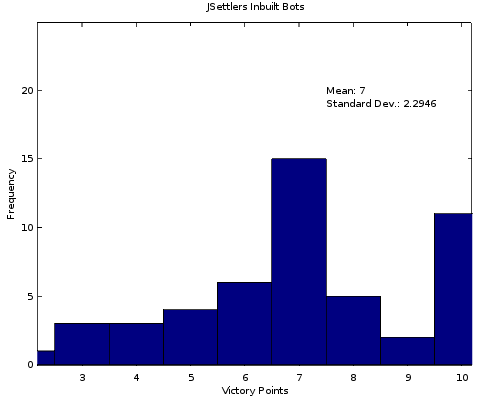
\includegraphics[width=0.75\linewidth]{figures/inbuilt.png}}
  \caption{Results of inbuilt JSettlers bots - 50 Games}
  \label{fig:inbuilt} 
\end{figure}
\end{center}

\par From the graph of the results of the games played with only the bots supplied with the JSettlers2 client we can see that the overall standard of play is quite strong with a mean score of 7. A standard deviation of about 2.3 indicates that there is some degree of inconsistency present in the JSettlers bot but this is not unexpectedly large and can be attributed to the random elements of the game.  

\par A further baseline that is worth establishing is the performance of a bot playing certain other strategies of interest so that they can be compared against the MCTS bot developed. There are two strategies that will be used to act as a comparison, random play and simple heuristic play, as utilised in the playout strategy for the simulator. The results of these strategies are as follows when played against the JSettlers bots.

\begin{center}
\begin{figure}[H]
 \centerline{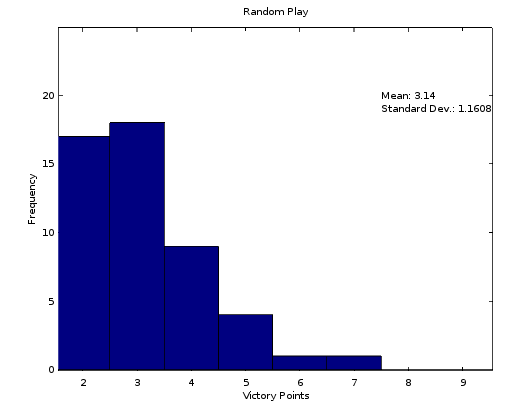
\includegraphics[width=0.75\linewidth]{figures/random.png}}
  \caption{Results of random play - 50 Games}
  \label{fig:random1} 
\end{figure}

\begin{figure}[H]
 \centerline{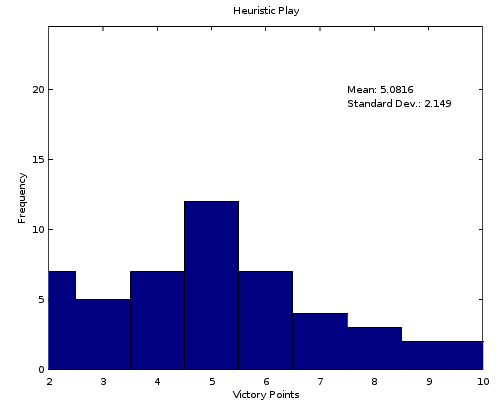
\includegraphics[width=0.75\linewidth]{figures/heuristic.png}}
  \caption{Results of simple heuristic play - 50 Games}
  \label{fig:heuristic1} 
\end{figure}
\end{center}

\par The graph show that random play is an ineffective strategy for playing Catan. Despite this, in the majority of random games that were played at least one point scoring action was made and only a minority of games ended with the minimum of two victory points that are obtained from placing the opening settlements. The random play utilised the heuristic opening strategy and it could be expected that play that was completely random it its execution would in fact perform even worse due to the likelihood of not getting enough resources to luckily gain a victory point.

\par On the other hand the heuristic approach that is utilised as a playout strategy by the simulator performs significantly better, even winning some games. However, this particular bot should not be considered particularly strong as it only averages a score of 5 victory points per game, a value that a competent human player should easily be able to match and beat. It is also relatively inconsistent with a high standard deviation meaning that although it can sometimes win games it is not uncommon to finish games with a very low amount of victory points. 

\subsection{Effects of Heuristic Opening Strategy}

At the start of the game of Catan the opening stage dictates where the first two settlements and roads for each player is placed. We approach this by using a heuristic opening strategy as detailed in the design section that takes into account the values of the tiles of resources and their resource type. In order to evaluate the effectiveness of this we compare 3 different playing styles (random, heuristic and MCTS with 1000 simulations) and examine the results achieved using a random starting strategy compared to one using the heuristics. 

\begin{figure}[H]
\centering
\begin{minipage}{.5\textwidth}
  \centering
  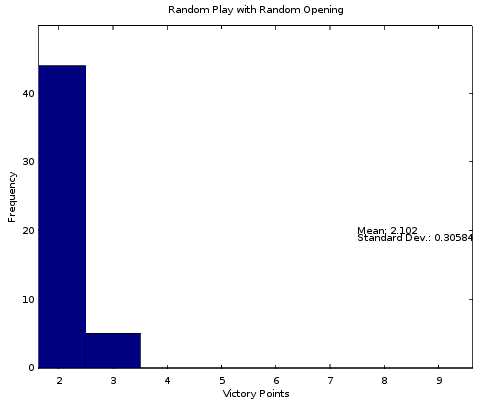
\includegraphics[width=.9\linewidth]{figures/roRandom}
  \captionof{figure}{Random Play with Random Opening}
  \label{fig:opening1}
\end{minipage}%
\begin{minipage}{.5\textwidth}
  \centering
  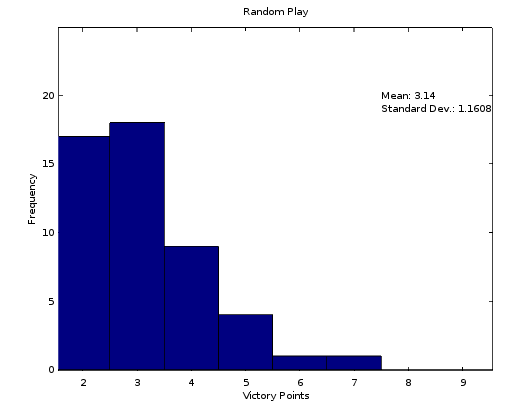
\includegraphics[width=.9\linewidth]{figures/hoRandom}
  \captionof{figure}{Random Play with Heuristic Opening}
  \label{fig:opening2}
\end{minipage}
\end{figure}

\begin{figure}[H]
\centering
\begin{minipage}{.5\textwidth}
  \centering
  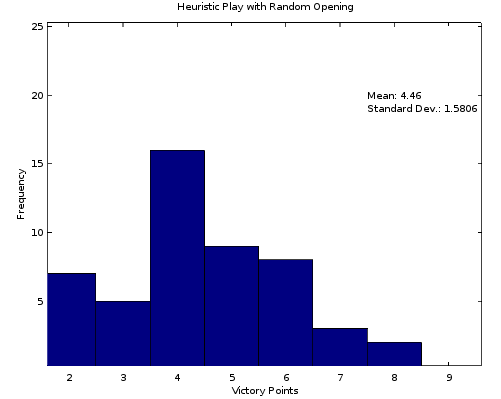
\includegraphics[width=.9\linewidth]{figures/roHeuristic}
  \captionof{figure}{Heuristic Play with Random Opening}
  \label{fig:opening3}
\end{minipage}%
\begin{minipage}{.5\textwidth}
  \centering
  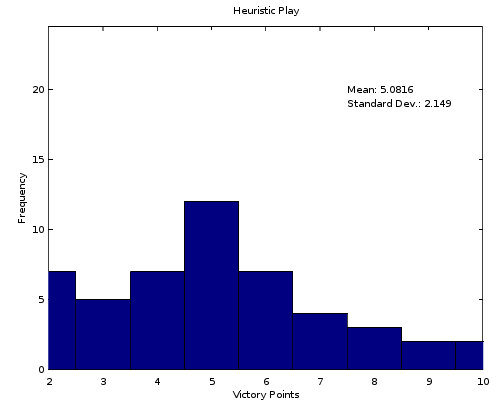
\includegraphics[width=.9\linewidth]{figures/hoHeuristic}
  \captionof{figure}{Heuristic Play with Heuristic Opening}
  \label{fig:opening4}
\end{minipage}
\end{figure}

\begin{figure}[H]
\centering
\begin{minipage}{.5\textwidth}
  \centering
  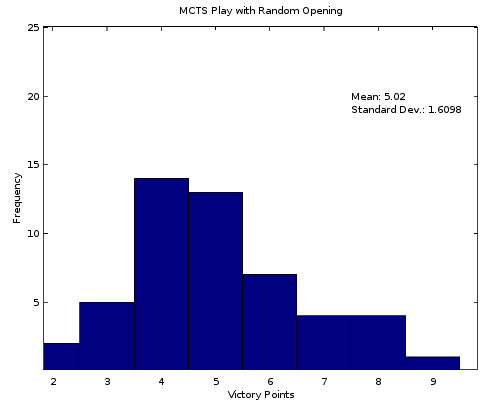
\includegraphics[width=.9\linewidth]{figures/roMCTS}
  \captionof{figure}{MCTS 1000 simulations with Random Opening}
  \label{fig:opening5}
\end{minipage}%
\begin{minipage}{.5\textwidth}
  \centering
  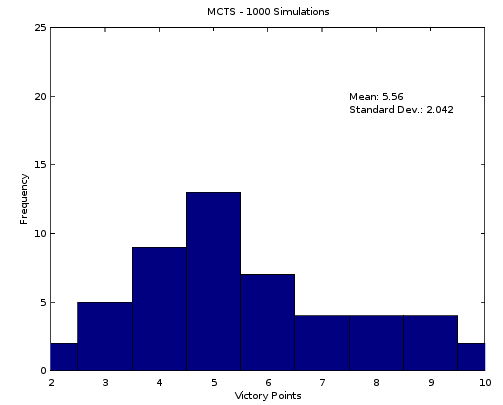
\includegraphics[width=.9\linewidth]{figures/hoMCTS}
  \captionof{figure}{MCTS 1000 simulations with Heuristic Opening}
  \label{fig:opening6}
\end{minipage}
\end{figure}

\par From the graphs we can see that the heuristic opening strategy gives a noticeable improvement to the playing ability of the bot when compared to random opening strategies. On average, the mean number of points scored increased by about 0.5 in the non-random strategies and by a more significant amount in random play. It also interesting to note that not a single game was won when the opening strategy was randomly determined, displaying the importance of the opening moves to the game. The standard deviation of the non-random strategies reflects this by increasing and the histograms showing a wider spread towards the right. 

\par The speed of the calculation of the opening strategy was also impressive, taking place almost instantly. This is a benefit when compared to MCTS which could take a significant amount of time to perform the required number of playouts.

\subsection{Effects of Adjustment of UCT Exploration Parameter}

During the selection stage of MCTS the UCT formula is used for picking the children of decision nodes. The UCT formula has a parameter, $c$, which determines the balance between exploration and exploitation in the search process. This parameter is domain specific and must be tuned manually. Efforts have been made to develop analytic methods in order to work out the optimal value of $c$ for particular games \autocite{chaslot2008cross, kozelek2009methods}, we will determine a good value of $c$ using an empirical approach by examining the performance of bots across a number of games using different values of the parameter.

\par In order to speed up the execution of the search for results a set of 50 games was played with 1000 Simulations per turn with a range of different $c$ parameters in order to try and find an acceptable value of $c$ for usage by our AI.

\begin{center}

\begin{figure}[H]
\centering
\begin{minipage}{.5\textwidth}
  \centering
  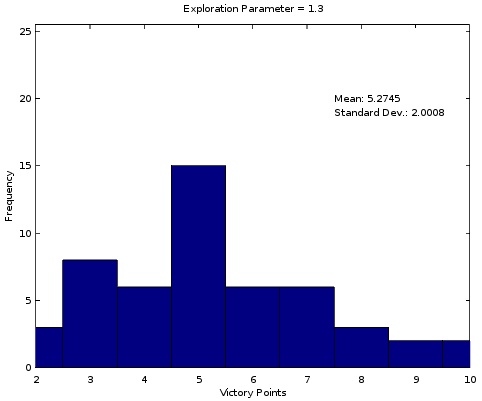
\includegraphics[width=.9\linewidth]{figures/exploration1-3}
  \captionof{figure}{Exploration parameter of 1.3}
  \label{fig:explore1.3}
\end{minipage}%
\begin{minipage}{.5\textwidth}
  \centering
  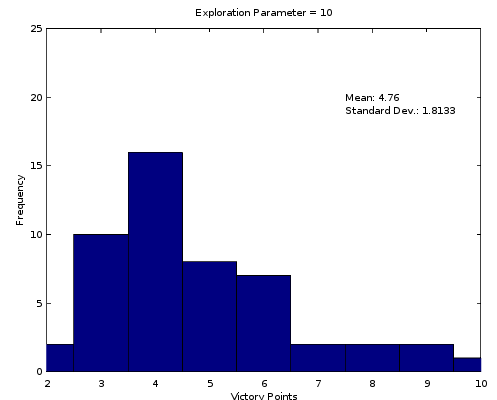
\includegraphics[width=.9\linewidth]{figures/exploration10}
  \captionof{figure}{Exploration parameter of 10}
  \label{fig:explore10}
\end{minipage}
\end{figure}

\begin{figure}[H]
 \centerline{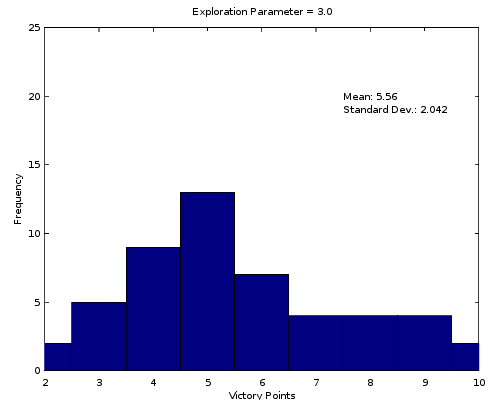
\includegraphics[width=0.75\linewidth]{figures/exploration3.png}}
  \caption{Exploration parameter of 3}
  \label{fig:explore3} 
\end{figure}
\end{center}

\par From these figures we can see that picking a higher exploration parameter such as 3 improves results over a lower one. However it must also be noted that if we increase the exploration parameter too high then performance will be drastically reduced. This is because if the exploration parameter is too high then very little exploitation of nodes that the simulator has indicated to be promising get explored meaning that information granted by the simulations is effectively ignored.

\par This value could undoubtedly be tuned further until an ideal value is found, perhaps using techniques such as cross validation as mentioned earlier. Another possible factor of the $c$ value is that it may beneficial to set it to different values depending on the time of the game, an idea proposed by \textcite{roelofs2012monte}. This idea may have some merit to as when games had a high exploration parameter they appeared to have a more consistent early game than those where exploitation of the existing nodes was valued more but struggled to progress much as the game drew on, a fact shown somewhat by the fact the standard deviation of the higher exploration values is lower than the other exploration parameters. An interesting development would be to adjust to $c$ parameter at particular times during the game and see if it could improve the standard of play.


\subsection{Effects of Adjustment of Simulation Count}

One of the key parameters of MCTS that affects the performance of the search is the number of simulations that are performed. In order to test this we had the bot play a set of games with varying numbers of maximum simulations per turn against the inbuilt AI of the JSettlers system. 

\begin{center}

\begin{figure}[H]
\centering
\begin{minipage}{.5\textwidth}
  \centering
  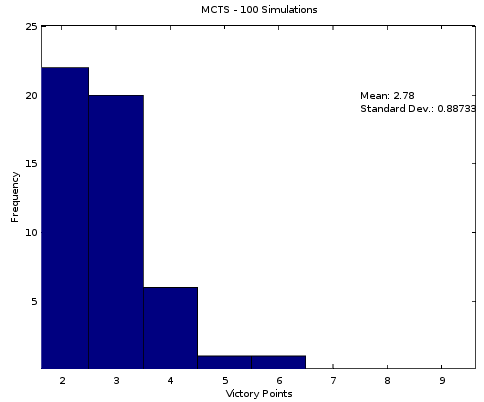
\includegraphics[width=.9\linewidth]{figures/mcts100}
  \captionof{figure}{Play with 100 Simulations}
  \label{fig:mcts100}
\end{minipage}%
\begin{minipage}{.5\textwidth}
  \centering
  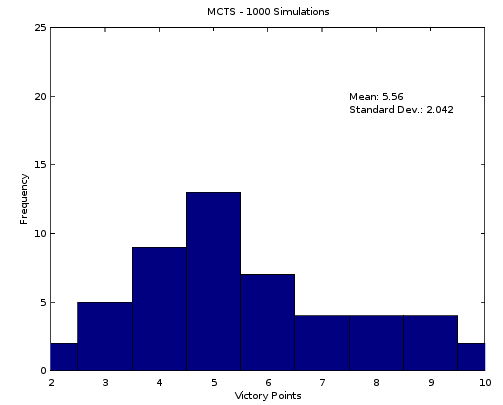
\includegraphics[width=.9\linewidth]{figures/mcts1000}
  \captionof{figure}{Play with 1000 Simulations}
  \label{fig:mcts1000}
\end{minipage}
\end{figure}

\begin{figure}[H]
 \centerline{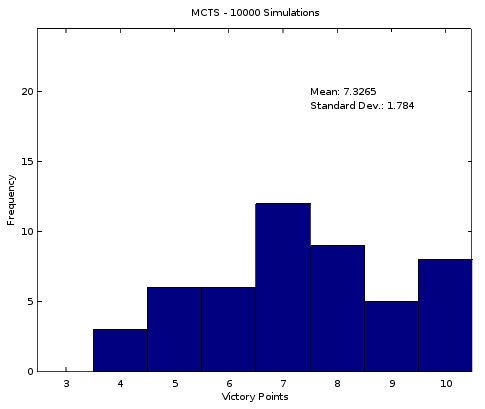
\includegraphics[width=0.75\linewidth]{figures/mcts10000}}
  \caption{Play with 10000 Simulations}
  \label{fig:mcts10000} 
\end{figure}
\end{center}

\par The graphs above indicate that, as expected, the adjustment of the number of simulations that are carried out drastically affects the strength of the play of the game. A game where only 100 simulations are used per turn results in very weak play, with the outcome comparable with random play. This could be explained by the fact that so few simulations are used not enough information is gathered by the simulator in order to make an informed decision. 

\par The ability of play jumps when the simulations per turn is increased to 1000. At this level the play could be considered about equal to the simple heuristics used as the policy for the play outs. With this level of simulation the time taken by the bot to process each move was fairly reasonable, taking around 10-20 seconds on an above average desktop computer with about 6GB of memory allocated to the execution environment of the program and a 3.4GHz processor. The time taken for the simulations decreased as the game went on, this is to be expected as fewer steps were needed by the simulator in order for the game to be concluded.

\par When the number of simulations was increased by a further factor of 10 the playing strength again improved, with the bot now able to regularly win games against the bots provided by the JSettlers software. The downside to this number of simulations was that the speed at which turns were carried out by the bot was now particularly slow, with a turn now often taking several minutes to process. Although this amount of time was tolerable when carrying out initial testing and gathering results it would not be fast enough to play in a fast paced AI game or to be acceptable when playing human opponents. However the results produced by this bot indicated that its playing strength was quite impressive.

\par It can be seen the performance of the bot increases in a linear fashion as the number of simulations rises by a factor of 10. Eventually, this will start to diminish as the maximum performance possible using this technique is attained.

\subsection{Play against Humans}
 
An aspect of AI systems that is often addressed is the ``humanness'' of their playing ability. This is a trait often discussed in Chess systems where an AI that plays in a similar nature to a strong human can be considered to be a good training aid. Incidentally it can also be seen that sometimes the accepted manner of high level of human play is not followed by bots, making some moves that would be considered by a regular player to be strange or unorthodox. 

\par It was seen as worthwhile to test the playing ability of the bot against human players. This would expose it to different playing styles as well as different levels of competence in its opposition. 

\par In each game where a human was used for testing the participant played in a game against one of the MCTS AI developed in this poject and two of the inbuilt AI that were present in the JSettlers game with the first move being assigned at random.

\subsubsection{Novice}
Against a novice player 5 games were played against an MCTS bot with maximum simulation count of 1000 and exploration constant of 3.

\par The novice player had only played Catan a few times before and needed some of the rules clarifying to them.

In these games the number of victory points distributed were as follows:

\begin{center}
\begin{tabular}{|c||c|c|c|c|}
\hline
Game & Human & MCTS AI & Inbuilt 1 & Inbuilt 2\\
\hline
1 & 5 & 5 & 10 & 9 \\
\hline
2 & 7 & 6 & 10 & 6 \\
\hline
3 & 4 & 8 & 7 & 10\\
\hline
4 & 7 & 7 & 8 & 10 \\
\hline
5 & 8 & 6 & 10 & 7 \\
\hline
\end{tabular}
\captionof{table}{Novice player against MCTS with 1000 simulations}
\end{center}

A single game against the MCTS bot with maximum simulation count of 10,000 was played. In this game the result was as follows: 

\begin{center}
\begin{tabular}{|c||c|c|c|c|}
\hline
Game & Human & MCTS AI & Inbuilt 1 & Inbuilt 2\\
\hline
1 & 6 & 8 & 6 & 10\\
\hline
\end{tabular}
\captionof{table}{Novice player against MCTS with 10000 simulations}
\end{center}

\par From these results it can be seen that when 1000 simulations per turn were utilised by the bot it performed about as well as a novice human player and when the number of these simulations went up it played a stronger game and generally seemed to outclass the novice human player. However the sample size from these games played was quite small meaning that detailed conclusions of the relative playing strength of the bot against novice humans cannot be accurately concluded from the numerical data provided.

\subsubsection{Expert}
In addition to playing against a novice player the developed AI system was also tested against the author of this project who considers himself an expert having played well over 150 games against a variety of different human and AI opponents of differing skill levels. A similar set up to the tests used for the novice player were used with one MCTS bot and two of the inbuilt bots used.

\par The tests again followed a similar pattern to before with 5 games of the MCTS simulation limit per turn set to 1,000 and a single game with the MCTS simulation limit per turn set to 10,000 

\begin{center}
\begin{tabular}{|c||c|c|c|c|}
\hline
Game & Human & MCTS AI & Inbuilt 1 & Inbuilt 2\\
\hline
1 & 8 & 8 & 10 & 9 \\
\hline
2 & 10 & 6 & 8 & 9 \\
\hline
3 & 7 & 5 & 7 & 10\\
\hline
4 & 6 & 5 & 10 & 7 \\
\hline
5 & 10 & 4 & 9 & 7 \\
\hline
\end{tabular}
\captionof{table}{Expert player against MCTS with 10000 simulations}
\end{center}

\begin{center}
\begin{tabular}{|c||c|c|c|c|}
\hline
Game & Human & MCTS AI & Inbuilt 1 & Inbuilt 2\\
\hline
1 & 7 & 9 & 6 & 10\\
\hline
\end{tabular}
\captionof{table}{Expert player against MCTS with 10000 simulations}
\end{center}

These results confirm that with simulation count of 1,000 the MCTS AI performs below the ability of an expert player. From these results it can also be seen that the inbuilt bots supplied by the JSettlers software seems to play at a very strong level. 


\subsection{Qualitative analysis of Play}
An interesting aspect of the bots play to consider is its style and strategy which can realistically only be evaluated by examining the bots playing games. For this qualitative analysis the bot was set to use a maximum number of simulations per turn of 10,000 with an exploration parameter of 3.

\par The analysis showed a number of interesting characteristics about the play of the bot. Firstly, the heuristic opening strategy employed seemed to repeatedly place the starting settlements in good positions on the board, ensuring that during the opening stages of the game a steady flow of resources were being received.

\par One aspect of play that performed worse than expected was the placement of roads. Often too many roads were placed in positions that were not optimal and sometimes the placement of roads was not done soon enough even if resources were available such that opponents were often able to make moves restriction expansion in the mean time. Another deficiency that seemed to be unearthed with the play of the bot was its weakness at ending the game when opportunities presented itself to it. There were a number of times where the bot could have played more convincing moves towards the end of the game

\par Despite these shortcomings in the playing style and strategies employed by the bot developed during in this project there were a number of positive features surrounding its play. It was able to play a strong early game, expanding its income of resources early on in the game. It was also able to spend its resources consistently, rarely ever holding onto too many so that it could be robbed if a 7 was rolled. The bot showed signs of strong human-like play but an experienced player would have been able to tell that it was a bot that was playing the game and also be able to beat a good amount of the time.

\section{Evaluation}
\subsection{Peformance}

On the whole, it can be seen that when the bot is played using the strongest viable configuration discovered by this project it is relatively strong. Results have shown that is is able to play against both novice and expert human player and achieve good results although it is not able to win the majority of the games that it takes part in. Even in games where the AI did not win it was able to produce a good score.

\subsection{Comparison with Other Systems}
The most obvious comparison that can be made is against the JSettlers AI that the bot developed during this project was thoroughly tested against. The JSettlers AI has been developed over a number of years and has reached a high standard of play. The MCTS approach used during this project performed strongly against this AI winning a good number of games and achieving a high average score in the games that it didn't win. If more simulations were possible and all other parameters and values were optimised it seems possible that the bot developed using the MCTS technique at its core would comfortably be able to beat this bot.

Comparisons could also be made against the system developed by \textcite{szita2009monte} which used the same API. Although at first glance the bot developed in that paper appears to comfortably beat the packaged AI in a larger proportion of the games it plays than the bot developed as a result of this project it must be taken into account that these experiments were carried out a significant amount of time ago. Since then, the bots included in the JSettlers package have received numerous upgrades and now appear to be considerably harder, a fact that is supported when the expert player in the paper believes that the bots included can be comfortably beaten by an expert human player. Currently, the JSettlers bots hold their own very well against an expert human player. Commits to the git repository where the JSettlers project is maintained confirm that numerous improvement have been made to the bot. For these reasons it would appear that comparisons against the Szita bot are quite hard to make as there is not a common baseline of the performance upon which to compare them. The same situation is true for all other papers found using the JSettlers project to play Catan as none have been completed particularly recently, making comparisons with them hard.  

\subsection{Limitations and Issues}
The main issue that impacted the performance and development of the system was the speed and accuracy of the simulator, given how closely it can be seen that the number of simulations performed is tied to the overall strength of play this could be a large issue. When testing, unlimited time was provided in order to allow the bot to make its moves. If the bot were forced to conduct its turns within a certain time frame then this may seriously impact the performance of the bot. 

\par Time taken to complete the simulation was not the only concern with available memory in the system also being able to pose problems if not enough was allocated to the execution environment. This situation could be easily rectified however, by changing the structure of the trees built by the program so that they are more resource efficient, and by allowing the system to use more memory.

\par When it came to the in game abilities of the bot there were not too many issues and play could generally considered to be strong, meeting the main aim set out for the project. However there were some areas where the play of the bot could have been improved after the qualitative analysis was given. One issue with the play of the bot was that it was ineffective when using development cards, often not playing them or using them at the wrong time. This was most likely down to a programming error in the implementation of the bot as the handling of these playing situations should be comfortably handled by the MCTS and its simulator capabilities. A further game playing issue was its lack of decisiveness at the end of games, shown by the way that it managed to achieve a high mean value of victory points but was not able to win a correspondingly high number of games. This could have been improved by modifying the MCTS to provide much greater weight to terminal moves or by implementing a variation of the end game book technique that is commonly implemented by Chess programs.

\par The only other significant issue that presented itself in the game playing ability of the bot was its road placement that at times, even on a high level of simulations proved to be suboptimal. Theoretically a large enough number of simulations should lead to greatly improved look ahead and the bot should place roads in beneficial positions, however in our case roads were often placed in positions that would not be helpful. On the whole, however, this did not have too much of a drastic impact on the performance of the bot.

\par A shortcoming of the evaluation was that we were not able to test the effectiveness of a MCTS based opening. This particular technique was not able to be introduced due to limitations in the programming of the search as well as the communications provided by the server. If able to carry out an MCTS opening conclusions could have been drawn of whether the heuristic approach offered a good alternative. From our findings however, we were able to see that the heuristic based opening provided a significant boost to the playing potential of the bot and started allowing the bot to win games.

\subsection{Possible Improvements}
Despite the success of this attempt to play Catan using a mixture of heuristic and MCTS techniques a number of improvements could be made in order to further strengthen this bot and address the issues that were mentioned earlier.

\par The main improvement that could be made would be to significantly upgrade the performance of the simulator so that a larger number of simulations in a shorter period of time could be carried out. This would have two main benefits. Not only would the strength of the AI increase as we have shown that a larger number of simulations tends to lead towards stronger play but we would also be able to test other aspects of play more efficiently, such as working out the optimal value of the $c$ parameter.

\par As discussed earlier the optimal value of the exploration parameter for the UCT formula $c$, would also need to be found to further improve this bot although it is highly likely that there is single value that is optimal throughout the game and it may be a good approach to see if varying this value can lead to improved performance.

\par The heuristics for a number of the aspects of the game could be improved. While the opening play heuristics generally result in effective moves being played there is always room for improvement and as long as the computational effort did not increase to an excessive level more information could be applied to this stage of the game in an attempt to get better results. Other heuristics that could be improved include the simulated wins given during the MCTS, the scores used to evaluate which roads are available to place and the heuristics used to guide the simulator. 

\par Another improvement that would mainly fall onto the performance side would be to improve the efficiency of the generation of available moves, especially when a large number of resources are possessed resulting in a large search space. Although efforts have been made to narrow this search space and improve the efficiency there are still issues with the ability to fully examine all possible roads that could be placed on a given turn. This could be addressed by either redesigning the search structures used to generate all available moves or by adopting the practice of grouping moves into groups that have similar outcomes.

\section{Conclusion}
In this project we have designed and implemented a bot that can play the board game Catan to a relatively strong level. We used a novel approach when designing this bot, building on previous work and combining strong domain knowledge of the environment through heuristics as well as expanding on earlier attempts to play this game using a MCTS technique.

When analysing the game and designing the solution that we would implement we found numerous complications with the game such as the difference between the opening moves compared to the rest of the game and the difficulty in easily formulating all of the available moves that can be played by a player on their turn due to the compound nature of them. We took these factors into account when designing the techniques that would play this game, utilising our expert knowledge in order to develop suitable heuristics in cases where the search technique employed for the rest of the game would not be usable. On top this we also designed an integrated simulator for the game that would allow us to run simulations of games in any given state to their conclusions by following a given strategy.

The MCTS explored the handling of uncertainty in game trees as well as the UCT formula and the setting or parameters. A main area of focus was the effect of increasing the number of simulations with respect to the outcome of the game. It could be seen that when the number of simulations increased the playing strength of the bot also increased at the cost of time required in order to run the simulations.

\subsection{Possible Future Work}
Following on from this work a number of possible future tasks and research associated could be conducted
\subsubsection{Trading}
Currently the bot doesn't play Catan to the full specification of the rules due to its inability to trade between players. Although it could play in a game where trading is occurring and simply refuse the requests this would probably weaken its position. Therefore a worthwhile future task would be to design a system where the bot could trade. In order to do this the bot would have to be able to evaluate whether a trade proposed by another player was worthwhile in addition to being able to make a trade towards other players that is beneficial to itself.

Once trading has been introduced it would probably be necessary to retune the other techniques in order to take advantage of the newly gained abilities that will be granted to the bot by being able to trade.

\subsubsection{MCTS Optimisation}
Although efforts have been made to tune the MCTS so that it makes the best decisions possible there is undoubtedly room for improvement in it still. Areas where considerable effort could be applied to the MCTS mainly involve the exploration parameter of the UCT formula and the playout strategy that is utilised by the simulator when running games. 

The UCT parameter was determined empirically and kept constant. It would interesting to investigate whether changing this parameter during a game could help the bot make better decisions. This would show that different stages of the game value a differing balance between exploration and exploitation of the search space available to it.

A the playout strategy utilised by the simulation aspect of the MCTS can affect the strength of play. The system currently uses a heuristic approach, making use of expert domain knowledge in order to facilitate the rapid playing of simulation games. A valuable future task would be to work out the optimal method of running these playouts. 

\subsubsection{Simulator Performance Optimisation}
As part of this project a bespoke simulator needed to be designed in order to ensure that games could be simulated with enough speed that a MCTS based was a viable option. Although the simulator was fast enough in order to allow the testing of the MCTS an increase in performance of the simulator would not only allow for stronger play as a result of more simulations but more time effective evaluations of various aspects of the bot.

\appendix
\section*{Appendix}
\subsection*{.zip File Structure}
The .zip file submitted has the following files contained within it:
\paragraph{JARFiles}Containing a selection of executable JAR files compiled fromt the source code fo this project. 
\paragraph{JSettlers}This directory contains the JAR and config files required to run the JSettlers software that acts as the game engine.
\paragraph{Report}Containing a copy of this report in PDF form.
\paragraph{SourceCode}Contains the full source code of the developed software

\vspace{2cm}

\subsection*{Running the Program}
The recommended method to run this program is to use the JAR files supplied in the zip file. This can be achieved by running it from the command line using the command \code{java -jar <filename>}. The JAR files have names which indicate what configuration they are running in. If running versions of the JAR that utilise MCTS, especially those with high simulation counts, it is highly recommended to allocate a large (at least 6GB) amount of RAM to the JVM and to force 64-bit mode to ensure better performance.  

\par In order to run software it will be necessary to start the JSettlers2 server, the JAR files for this can be found in the \textit{JSettlers} directory. Again the \code{java -jar <filename>} should be used. Do not edit the port the server runs on or the cookies used by the bots as this 
will cause the project bot to fail to connect. Automatic bot games will start in 15 seconds unless they are disabled. This is the window in which to start the bot and connect it to the server.

\par The client can be started in a similar manner and allows the user to spectate games or play against the bot. Included is a properties file which must be in the same directory as the the server executable. This properties file can be edited to change the nature of the game. Of interest to edit is the \code{jsettlers.bots.botgames.total} property which enables automatic bot games. Set this number to a negative value if you wish to play against the bot as a human. Full details of these properties and details for running the JSettlers server and client are in the readme files in the \textit{JSettlers} directory.

\par Compilation from source is not recommended as the JSettlers2 project source code needs to be placed on the classpath. This source code is available from https://github.com/jdmonin/JSettlers2.

\par The project bot and the server is at times unstable and may crash occasionally despite best efforts. If this happens restart both the server and the bot.
\printbibliography

\end{document}